\documentclass[border=10pt]{standalone}
\usepackage{pgfplots}
\pgfplotsset{compat=1.17}
\begin{document}
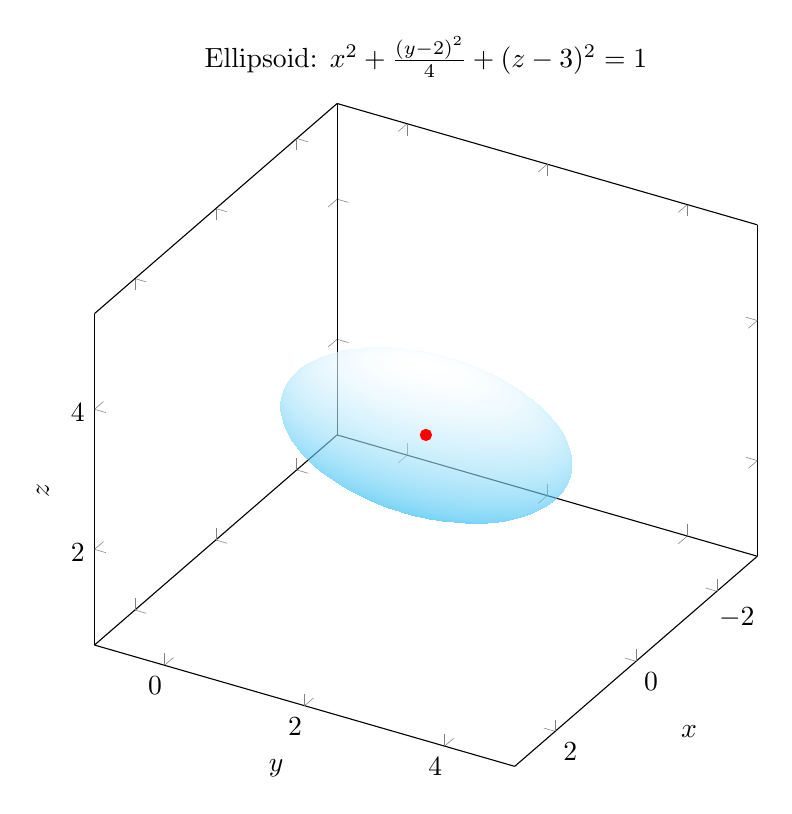
\begin{tikzpicture}
\begin{axis}[
    view={120}{30},
    xlabel=$x$, ylabel=$y$, zlabel=$z$,
    xmin=-2, xmax=2,
    ymin=-1, ymax=5,
    zmin=1, zmax=5,
    width=10cm, height=10cm,
    axis equal,
    title={Ellipsoid: $x^2+\frac{(y-2)^2}{4}+(z-3)^2=1$}
]
\addplot3[
    surf,
    shader=interp,
    opacity=0.6,
    colormap={cyanwhite}{color=(cyan) color=(white)},
    domain=0:360,
    y domain=0:180,
    samples=40,
    z buffer=sort
]
({sin(y)*cos(x)}, {2*sin(y)*sin(x)+2}, {cos(y)+3});
\addplot3[only marks, mark=*, red] coordinates {(0,2,3)};
\end{axis}
\end{tikzpicture}
\end{document}
